\documentclass[professionalfonts]{beamer}
\newif\ifita
\itatrue % comment out to hide answers
%\itafalse
\usepackage[familydefault,light]{Chivo} 
\usepackage[T1]{fontenc}
\usenavigationsymbolstemplate{}
\usepackage[]{hyperref}
\usepackage{tikz,pgf,pgfarrows,pgfnodes,pgfbaseimage}
\graphicspath{{./Pics/}}
\usetikzlibrary{shapes}
\usepackage{setspace}
\newcommand{\evi}[1]{{\colorbox{yellow!50}{{#1}}}}
\newcommand{\exe}[1]{{\color{black!50}{{#1}}}}
\newcommand{\kw}[1]{{\colorbox{black!30}{\color{white}{#1}}}}
\tikzstyle{nd}=[circle,draw=black,thick,minimum size=.8cm,inner sep=1pt]
\setbeamercovered{transparent}
\usetheme{Singapore}
\tikzstyle{nodo}=[ellipse,draw=black!60,fill=black!10,line width=.7pt,minimum width=.7cm,minimum height=.4cm]
\usecolortheme[named=gray]{structure}
\setbeamercolor{block title}{bg=black!20,fg=black}
\setbeamercolor{block body}{bg=black!10,fg=black}

%%%%%%%%%%%%%%%%%%%%%
\ifita
\title{Algoritmi Numerici (Parte III)}
\subtitle{[Lezione 4 e 5] Metodi Approssimati}
\else
\title{Numerics (Part III)}
\subtitle{[Lecture 4 and 5] Approximate Methods}
\fi
\date{}
\author{Alessandro Antonucci\\{\tt alessandro.antonucci@supsi.ch}}
%%%%%%%%%%%%%%%%%%%%%%%%%%%%
\begin{document}
\maketitle

\frame{\frametitle{\ifita Esempio scalare \else Scalar (Useless) Version of our Ideas\fi}
\begin{columns}
    \begin{column}[]{0.6\textwidth} 
\begin{itemize}\pause
    \item \ifita Equazione Lineare \else Linear equation \fi $5 \cdot x = 7$ 
    \pause\item \ifita Decomposizione per differenza \else Decomposing the coefficient by difference \fi $5 = 8 - 3$
    \pause\item \ifita riscrivo \else Equation rewrites as \fi $8 \cdot x = 3 \cdot x + 7$
    \pause\item \ifita Divido per il coefficiente \else Divide by (left) coefficient \fi $x = \frac{3}{8} \cdot x + \frac{7}{8}$
    \pause\item \ifita Ricorsione \else Recursive view \fi $x_{j+1} = \frac{3}{8} \cdot x_j + \frac{7}{8}$
    \end{itemize}
    \end{column}
    \begin{column}[]{0.4\textwidth} 

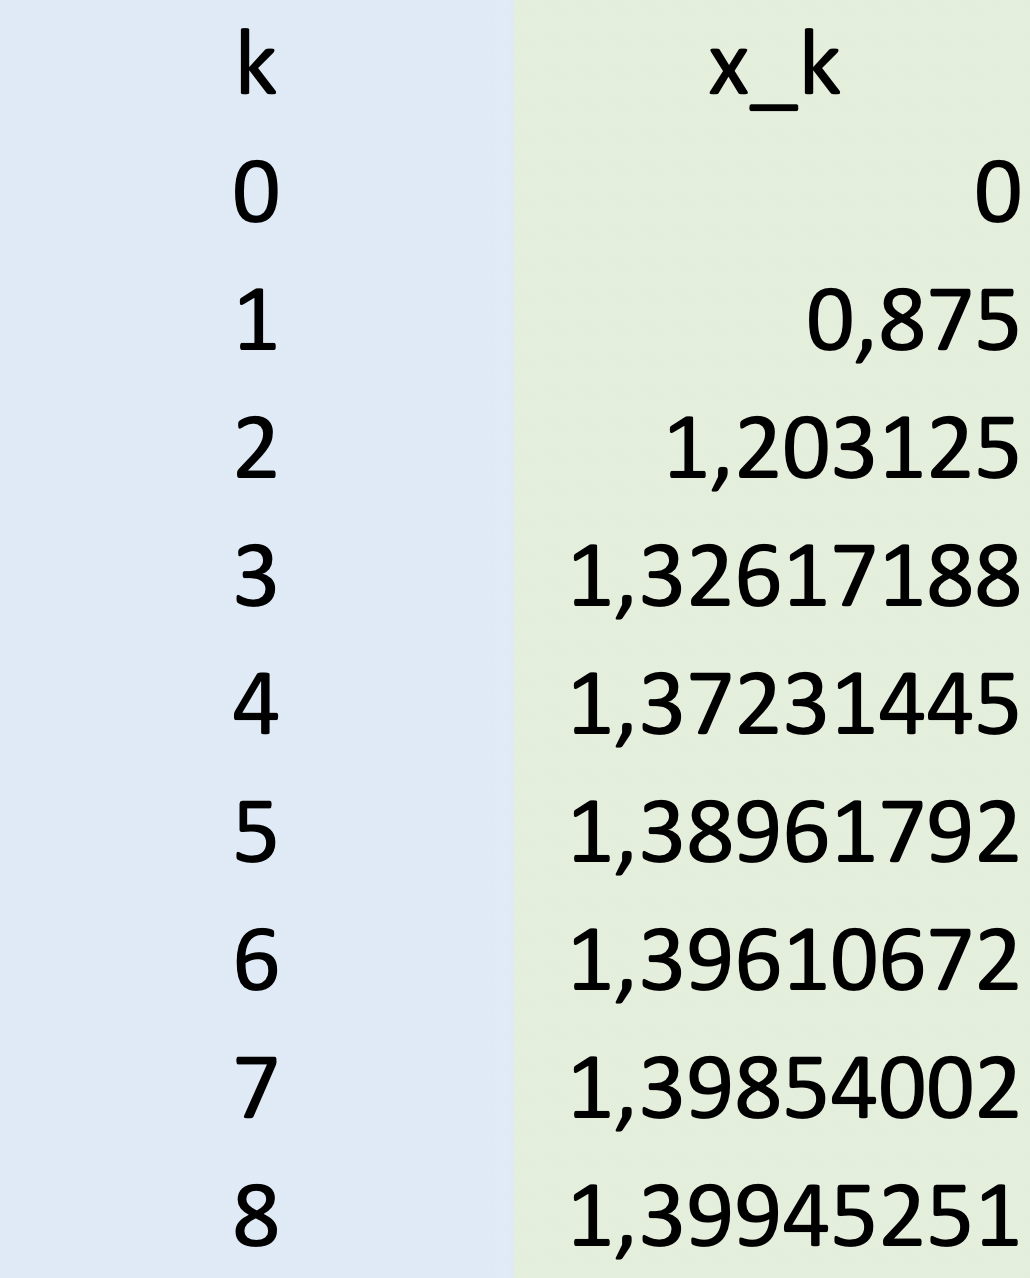
\includegraphics[width=3cm]{rec}
\end{column}
\end{columns}

}


\frame{\frametitle{\ifita Metodi Iterativi (Approssimati) \else Iterative Methods (Approx)\fi}
\begin{itemize}
\item \ifita Sistema lineare \else Given linear system \fi $\hat{A} \cdot \vec{x} = \vec{b}$
\item \ifita Scompongo matrice coefficienti per differenza \else
Decomposing coefficients' matrix by difference
\fi
$$\hat{A} = \hat{M}-\hat{N}$$
\item \ifita Il sistema diventa \else System rewrites as \fi  $\hat{M}\cdot \vec{x} = \hat{N} \cdot \vec{x} + \vec{b}$
\item 
\ifita Assumo $\hat{M}$ sia facilmente invertibile, $\hat{M}^{-1}$ nota
\else Assume $\hat{M}$ easy to invert, $\hat{M}^{-1}$ known
\fi
\item \ifita Il sistema diventa \else System rewrites as \fi $\vec{x} = \hat{M}^{-1} \cdot \hat{N} \cdot \vec{x} + \hat{M}^{-1} \cdot \vec{b}$
\item \ifita
Questa relazione pu\`o essere vista ricorsivamente:
\else
The relation can be seen as a recursion
\fi
$$\vec{x}_{n+1} = \hat{P}\cdot \vec{x}_n + \vec{q}$$
\ifita con \else where \fi$\hat{P}:=\hat{M}^{-1}\cdot \hat{N}$,  $\vec{q}:=\hat{M}^{-1}\cdot \vec{b}$
\end{itemize}}

\frame{\frametitle{\ifita Il metodo di Jacobi \else Jacobi's Method\fi}
\begin{itemize}
\item 
\ifita
$\hat{M}$ facile da invertire? Prendiamo $\hat{M}$ diagonale!
\else
$\hat{M}$ easy to invert? Let's take $\hat{M}$ diagonal!
\fi
\item \ifita Matrici diagonali sono banalmente invertibili \else Diagonal matrices are easy to invert \fi
\vskip 2mm
\begin{itemize}
\item \ifita L'inversa di una matrice diagonale \`e diagonale e sulla diagonale ci sono i reciproci \else The inverse of a diagonal matrix is diagonal too and has on its diagonal the reciprocal of the original elements
\fi
\end{itemize}
\item Jacobi? $\hat{M}$ 
\ifita diagonale e sulla diagonale elementi di 
\else diagonal with the (diagonal) elements of 
$\hat{A}$ \fi
\item \ifita L'algoritmo di Jacobi ha complessit\`a quadratica \else
Jacobi's algorithm has quadratic complexity
\fi
\item \ifita Prodotto $\hat{P}:=\hat{M}^{-1} \cdot \hat{N}$ veloce perch\'e $\hat{M}^{-1}$ \`e diagonale \else
Product $\hat{P}:=\hat{M}^{-1} \cdot \hat{N}$ fast because $\hat{M}^{-1}$ diagonal
\fi
\begin{itemize}
\item \ifita il prodotto di una matrice diagonale per una matrice qualunque si ottiene moltiplicando le righe della seconda per gli elementi corrispondenti della diagonale della prima \else
the product of a diagonal matrix by a generic matrix can be achieved by multiply the row of the second matrix by the corresponding diagonal elements of the first\fi
\end{itemize}
\end{itemize}}

\frame{\frametitle{\ifita Il metodo di Gauss-Seidel \else Gauss-Seidel Method\fi}
\begin{itemize}
\item \ifita Dato un sistema lineare \else Given a linear system \fi $\hat{A} \cdot \vec{x} = \vec{b}$
\item \ifita Scompongo la matrice dei coefficienti per differenza 
\else Decompose the coefficients' matrix as a difference \fi
$$\hat{A} = \hat{M}-\hat{N}$$
\item \ifita Il sistema diventa quindi \else The system becomes \fi $\hat{M}\cdot \vec{x} = \hat{N} \cdot \vec{x} + \vec{b}$
\item \ifita Questa relazione pu\`o essere vista ricorsivamente \else The relation can be seen as a recursion \fi
$$\hat{M} \cdot \vec{x}_{n+1} = \hat{N}\cdot \vec{x}_n + \vec{b}$$
\item 
\ifita
Dato $\vec{x}_n$ posso calcolare il secondo membro\\(ovvero i termini noti di un sistema)
\else
Given $\vec{x}_n$ compute the right-hand side\\(that is the constant array of the system)
\fi
\item 
\ifita
Se $\hat{M}$ \`e triangolare il sistema si risolve per sostituzione\\(complessit\`a quadratica)
\else
With triangular $\hat{M}$ system solved by substitution (quadratic complexity)
\fi
\end{itemize}}

\frame{\frametitle{\ifita Un esempio dimostrativo \else A demonstrative example \fi}
\begin{itemize}
\item \ifita Risolvere il sistema \else Solve the system \fi $\hat{A}\cdot \vec{x}=\vec{b}$ \ifita con: \else where: \fi
$$\hat{A} = \left[ \begin{array}{cc} 3 & -1 \\ 1 & -2\\ \end{array} \right],\quad
\vec{b} = 
\left[ \begin{array}{c} 1 \\ 1 \end{array} \right]$$
\ifita usando: \else by using: \fi
\begin{itemize}
\item \ifita due iterazioni dell'algoritmo di Jacobi \else two iterations of Jacobi's algorithm\fi
\item \ifita due iterazioni di Gauss-Seidel \else two iterations of Gauss-Seidel's algorithm\fi 
\end{itemize}
\vskip 2mm
\item \ifita In entrambi i casi usare l'inizializzazione: \else In both cases use the initialization: \fi
$$\vec{x}_0 = \left[ \begin{array}{c} 0 \\ 0 \end{array}\right]$$
\end{itemize}
}

\frame{\frametitle{\ifita Un esempio dimostrativo (Jacobi) \else A demonstrative example (Jacobi) \fi}
\begin{itemize}
\item $\hat{A} = \left[ \begin{array}{cc} 3 & -1 \\ 1 & -2\\ \end{array} \right]
= \hat{M} - \hat{N} = 
\left[ \begin{array}{cc} 3 & 0 \\ 0 & -2\\ \end{array} \right]-
\left[ \begin{array}{cc} 0 & 1 \\ -1 & 0\\ \end{array} \right]$
\item $\hat{M}^{-1} = \left[ \begin{array}{cc} \frac{1}{3} & 0 \\ 0 & -\frac{1}{2}\\ \end{array} \right]$
\item $\hat{P}:=\hat{M}^{-1}\cdot \hat{N} =  \left[ \begin{array}{cc} \frac{1}{3} & 0 \\ 0 & -\frac{1}{2}\\ \end{array} \right] \cdot
\left[ \begin{array}{cc} 0 & 1 \\ -1 & 0\\ \end{array} \right] = 
\left[ \begin{array}{cc} 0 & \frac{1}{3} \\ \frac{1}{2} & 0\\ \end{array} \right]$
\item $\vec{q}:=\hat{M}^{-1}\cdot \vec{b} =  \left[ \begin{array}{cc} \frac{1}{3} & 0 \\ 0 & -\frac{1}{2}\\ \end{array} \right] \cdot
\left[ \begin{array}{c} 1 \\ 1\\ \end{array} \right] = 
\left[ \begin{array}{c} \frac{1}{3} \\ -\frac{1}{2}\\ \end{array} \right]$
\item $\vec{x}_1 = \hat{P}\vec{x}_0 + \vec{q} = \vec{q} = \left[ \begin{array}{c} \frac{1}{3} \\ -\frac{1}{2}\\ \end{array} \right]$
{\it ( $\vec{x}_0=\left[ \begin{array}{c} 0\\ 0 \end{array} \right]$)}
\item $\vec{x}_2 = \hat{P}\vec{x}_1 + \vec{q} =
\left[ \begin{array}{cc} 0 & \frac{1}{3} \\ \frac{1}{2} & 0\\ \end{array} \right]
\left[ \begin{array}{c} \frac{1}{3} \\ -\frac{1}{2}\\ \end{array} \right]+
\left[ \begin{array}{c} \frac{1}{3} \\ -\frac{1}{2}\\ \end{array} \right] = 
\left[ \begin{array}{c} \frac{1}{6} \\ -\frac{1}{3}\\ \end{array} \right] $
\end{itemize}}

\frame{\frametitle{\ifita Un esempio dimostrativo (Gauss-Seidel) \else A demonstrative example (Gauss-Seidel) \fi}
\begin{itemize}
\item $\hat{A} = \left[ \begin{array}{cc} 3 & -1 \\ 1 & -2\\ \end{array} \right]
= \hat{M} - \hat{N} = 
\left[ \begin{array}{cc} 3 & -1 \\ 0 & -2\\ \end{array} \right]-
\left[ \begin{array}{cc} 0 & 0 \\ -1 & 0\\ \end{array} \right]$
\vskip 2mm
\item $\hat{M} \cdot \vec{x_1} = \hat{N} \cdot \vec{x_0} + \vec{b} = \vec{b}$ {\it ( $\vec{x}_0$ \ifita \`e il vettore nullo \else is the null vector \fi)}
\vskip 2mm
$\left[ \begin{array}{cc} 3 & -1 \\ 0 & -2\\ \end{array} \right] \cdot \vec{x}_1 = 
\left[ \begin{array}{c} 1 \\ 1 \\ \end{array} \right]
\Rightarrow
\vec{x}_1 = 
\left[ \begin{array}{c} \frac{1}{6} \\ -\frac{1}{2} \\ \end{array} \right]$
\vskip 2mm
\item $\hat{M} \cdot \vec{x_2} = \hat{N} \cdot \vec{x_1} + \vec{b} = 
\left[ \begin{array}{cc} 0 & 0 \\ -1 & 0\\ \end{array} \right] 
\left[ \begin{array}{c} \frac{1}{6} \\ -\frac{1}{2} \\ \end{array} \right] + 
\left[ \begin{array}{c} 1 \\ 1 \\ \end{array} \right]=
\left[ \begin{array}{c} 1 \\ \frac{5}{6} \\ \end{array} \right]$
\vskip 2mm
$\left[ \begin{array}{cc} 3 & -1 \\ 0 & -2\\ \end{array} \right] \cdot \vec{x}_2 = 
\left[ \begin{array}{c} 1 \\ \frac{5}{6} \\ \end{array} \right]
\Rightarrow
\vec{x}_2 = 
\left[ \begin{array}{c} \frac{7}{36} \\ -\frac{5}{12} \\ \end{array} \right]$
\end{itemize}}


\frame{\frametitle{\ifita Rilassamento Gauss-Seidel \else Relaxing Gauss-Seidel \fi}
\begin{itemize}
\item \ifita Data la soluzione di Gauss-Seidel \else Given Gauss-Seidel solution \fi $\vec{x}_1^{\mathrm{GS}}$ 
\item \ifita Posso combinarla con la soluzione precedente $\vec{x}_0$ per favorire la convergenza \else I can combine it with the previous solution $\vec{x}_0$ to improve convergence \fi
\item \ifita L'algoritmo diventa quindi \else The algorithm becomes \fi
\begin{itemize}
\item $\vec{x}_1^{\mathrm{GS}}$ tale che $M \vec{x}_1^{\mathrm{GS}} = N \vec{x}_0 + \vec{b}$
\item $\vec{x}_1 = \omega \vec{x}_1^{\mathrm{GS}} + (1-\omega) \vec{x}_0$
\end{itemize}
\end{itemize}

}

\end{document}
